%!TEX root = ../Dimensionieren I.tex

\section{Vor- \& Nachteile} % (fold)
	Vorteile:
	\begin{enumerate}
		\item Unterschiedliche Werkstoffe kombinierbar.
		\item Krafteinleitung wird gut verteilt.
		\item Geringes Gewicht.
		\item Gute Dämpfung gegen Körperschall.
	\end{enumerate}
	Nachteile:
	\begin{enumerate}
		\item Schälbeanspruchung verhindern!
		\item Kostenintensive Montage.
		\item Klabstoff muss Festigkeiten unter allen Betriebsbedingungen erfüllen.
	\end{enumerate}
% section: Vor- \& Nachteile (end)
\section{Festigkeit} % (fold)
	Verminderung der Festigkeit durch:
	\begin{tightitemize}
		\item Temperatur $>$ Einsatztemp.
		\item Bauteil zu glatt.
		\item Alterung
		\item Verunreinigungen
		\item Oberflächenbehandlung des Bauteils (eloxiert, verchromt, \dots)
	\end{tightitemize}
% section: Festigkeit (end)
\section{Gliederung} % (fold)
	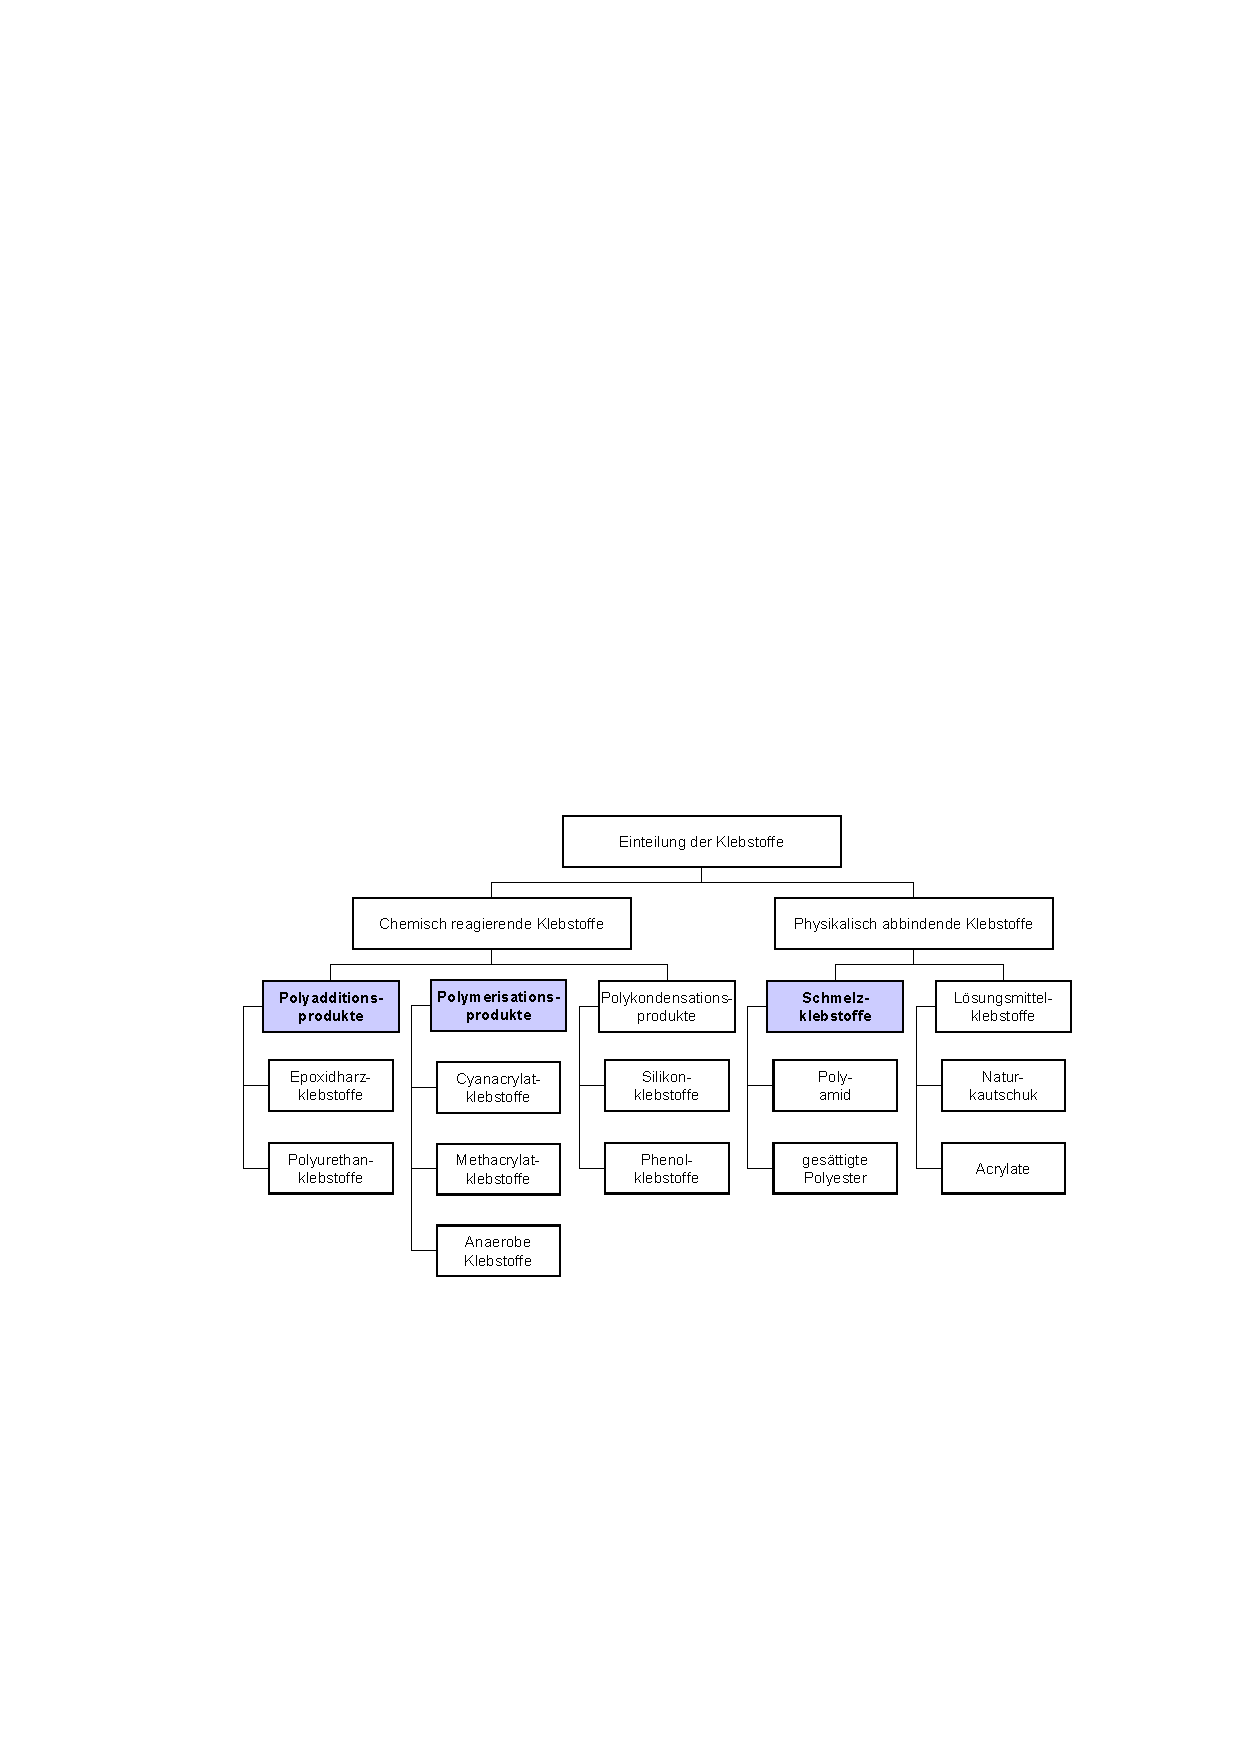
\includegraphics[width=\columnwidth]{graphics/klebstoffe}
	
	% \paragraph{Chemisch reagierende Klebstoffe}~ % (fold)
	% 
	% \small{
	% 	\begin{tabular}{lllll}
	% 		\toprule
	% 		\textbf{Klebertyp} & \textbf{Querkontrak-} & \textbf{E-Modul} & \textbf{Gleitmodul} & \textbf{Zugscherfestigkeit} \\
	% 		& \textbf{tionszahl} & $\unit{\mega\pascal}$ & $\unit{\mega\pascal}$ & $\unit{\mega\pascal}$ \\
	% 		\midrule
	% 		Warmhärtender & $0.38 - 0.40$ & $3000 - 4200$ & $900 - 1520$ & $20 - 35$ \\
	% 		Kalthärtender & $0.38 - 0.40$ & $1500 - 2500$ & $1500 - 2500$ & $18 - 25$ \\
	% 		\bottomrule
	% 	\end{tabular}
	% 	}
	% % paragraph: Chemisch reagierende Klebstoffe (end)
% section: Gliederung (end)
\section{Dimensionierung} % (fold)
	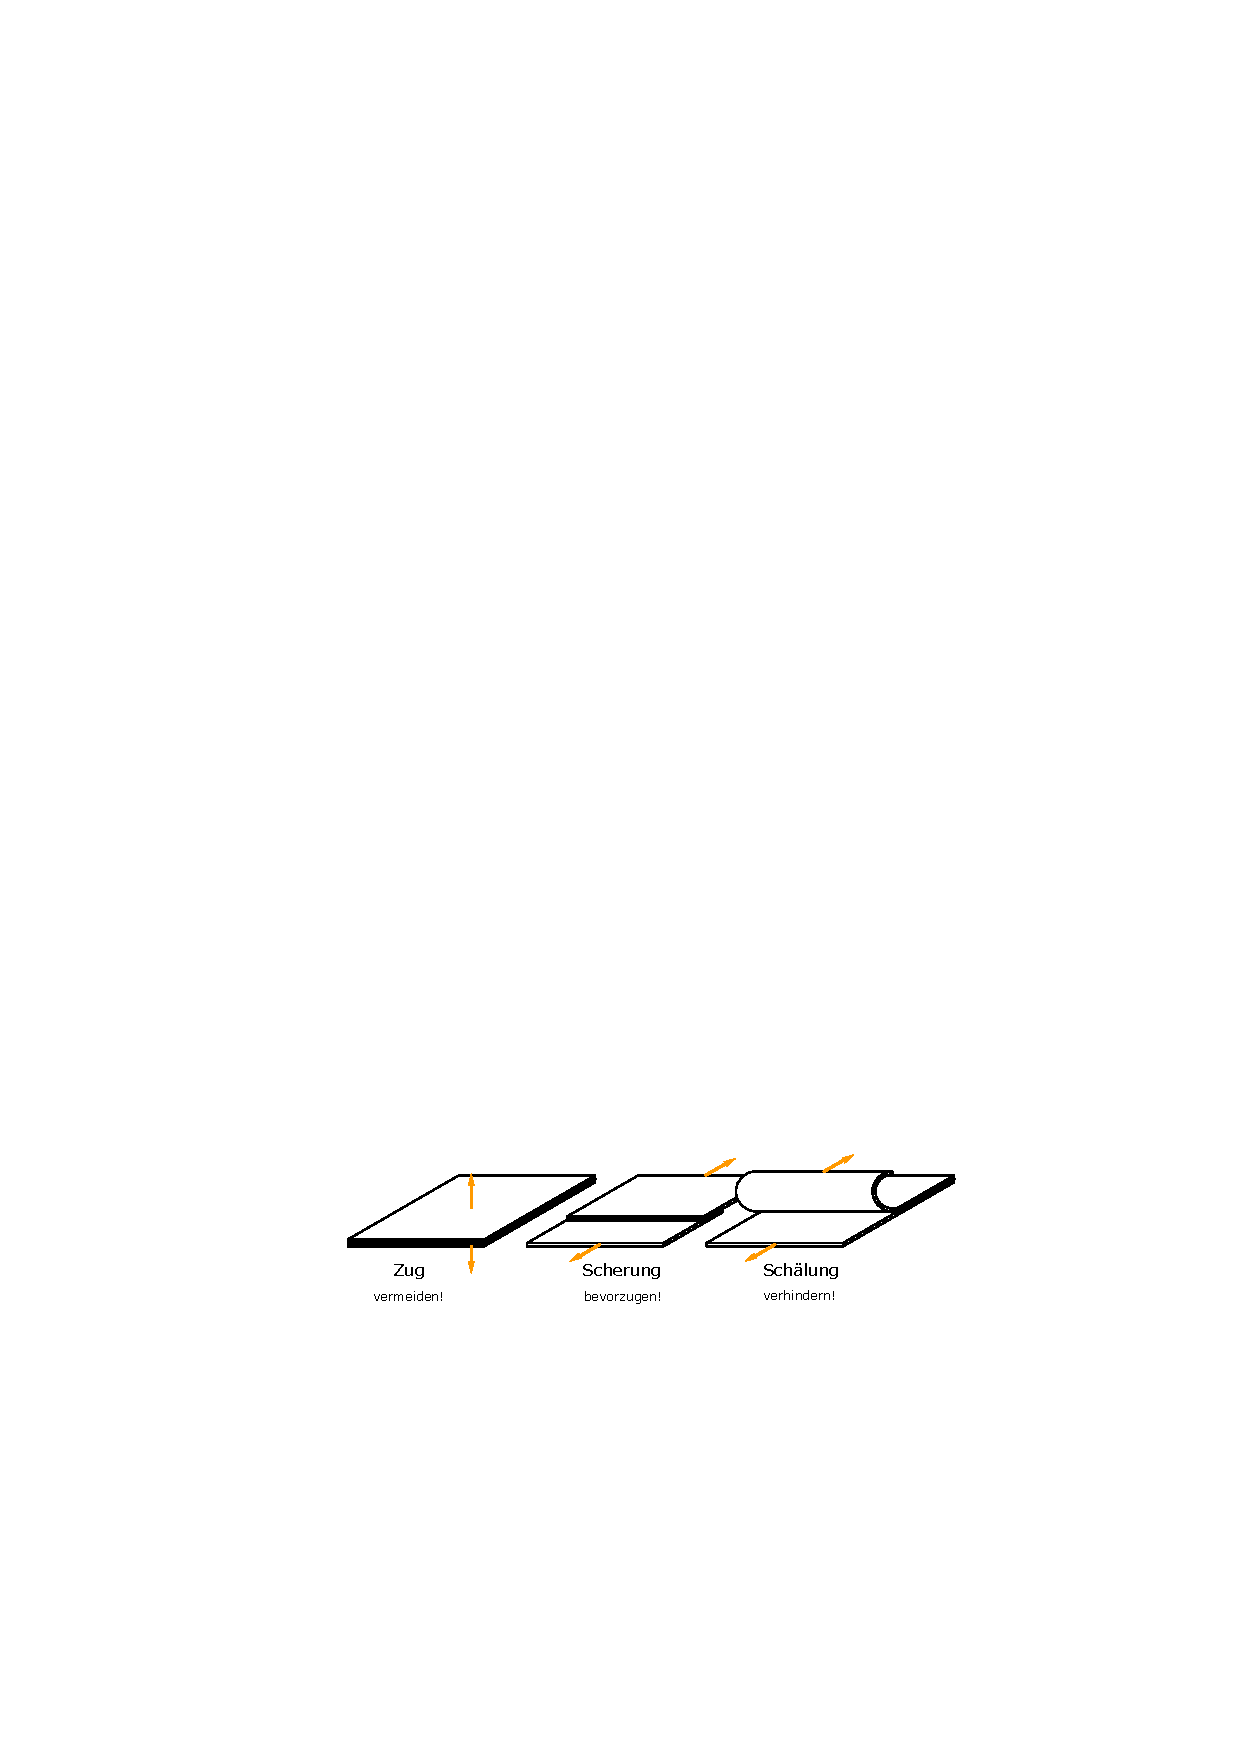
\includegraphics[width=\columnwidth]{graphics/klebstoffe_dimensionierung}

	\subsection{Zug/Druck-Beanspruchung} % (fold)
		\begin{wrapfigure}[0]{r}{.45\columnwidth}
			\vspace{-1.2cm}
			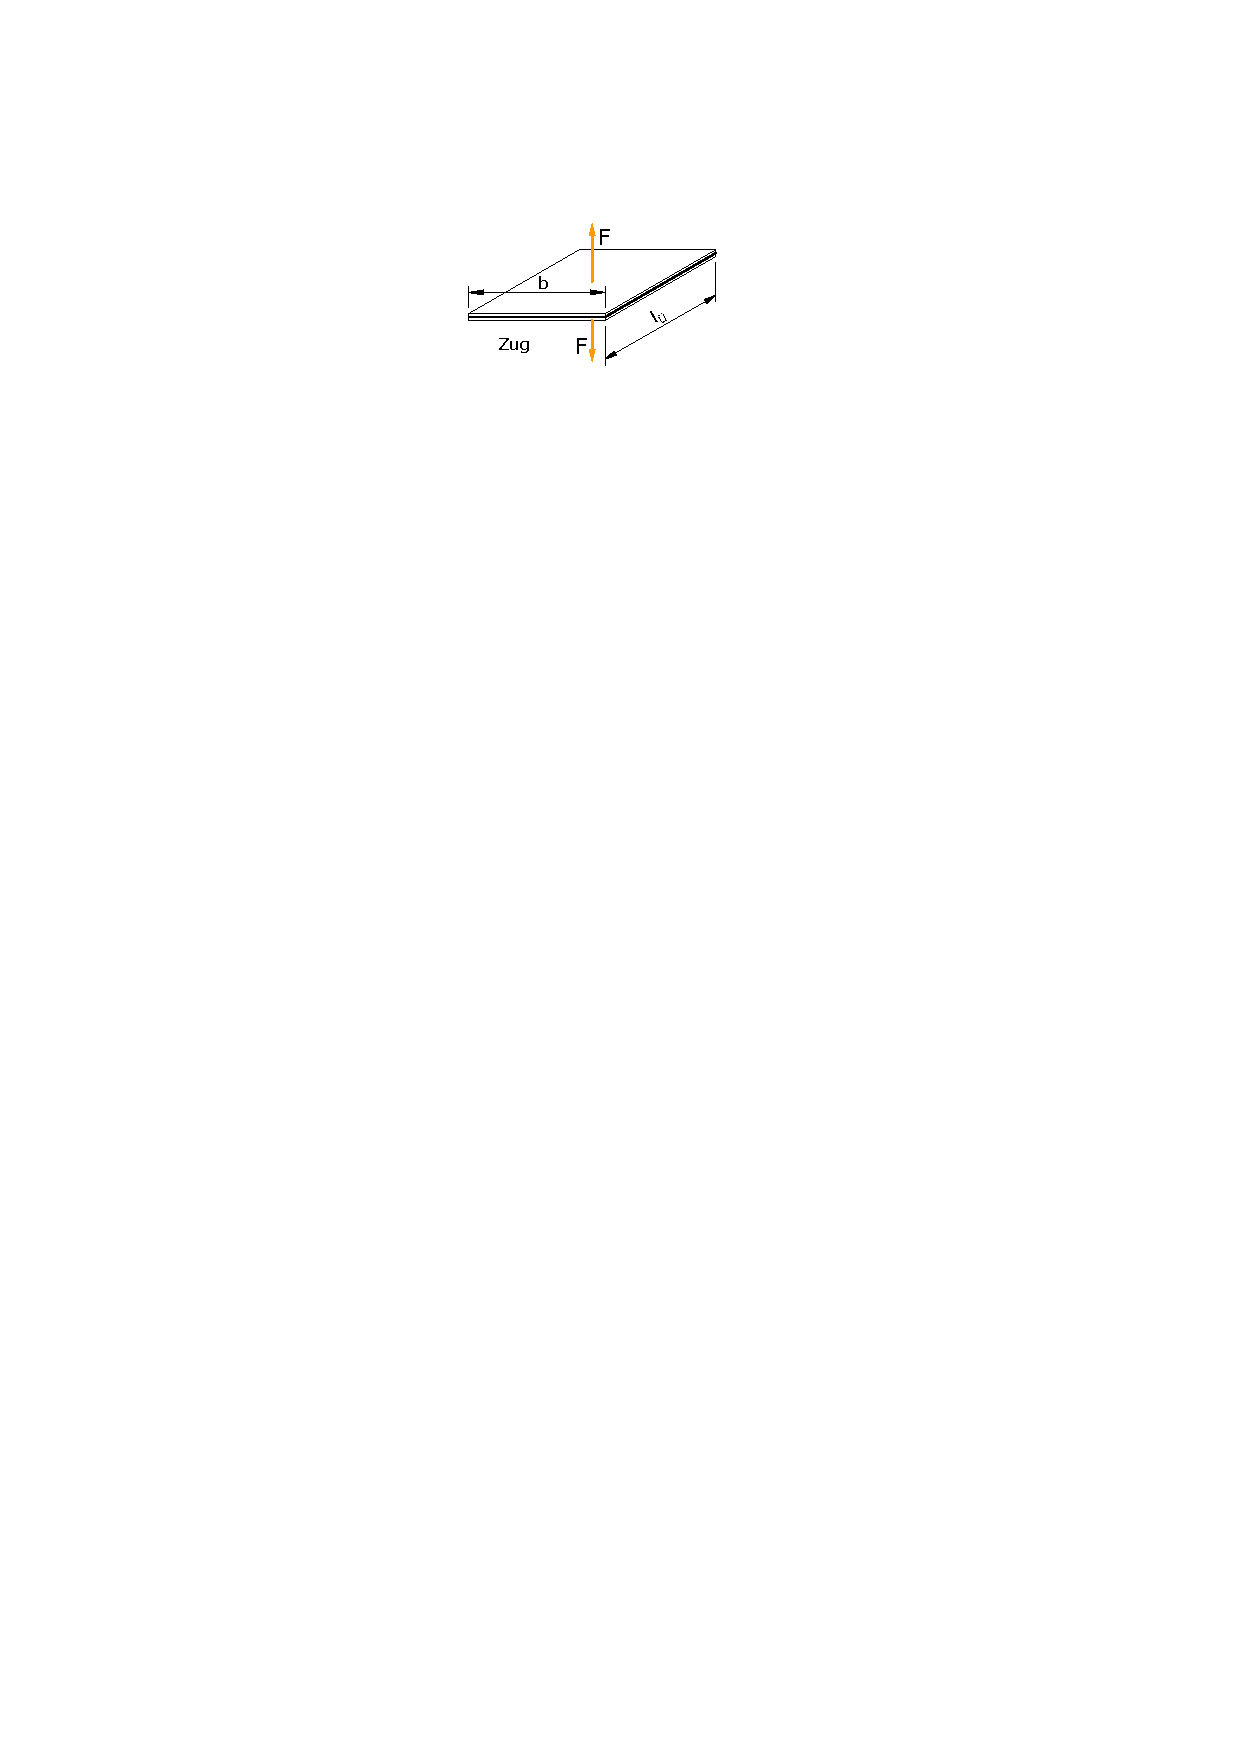
\includegraphics[width=.45\columnwidth]{graphics/klebe_zug}
		\end{wrapfigure}
		
		\begin{equation*}
			\sigma_x = \frac{F}{b \cdot l_{"u}} \leq \sigma_{\text{zul}}= \frac{\sigma_B}{S_B}
		\end{equation*}
	% subsection: Zug/Druck-Beanspruchung (end)
	\subsection{Scherbeanspruchung} % (fold)
		\begin{center}
			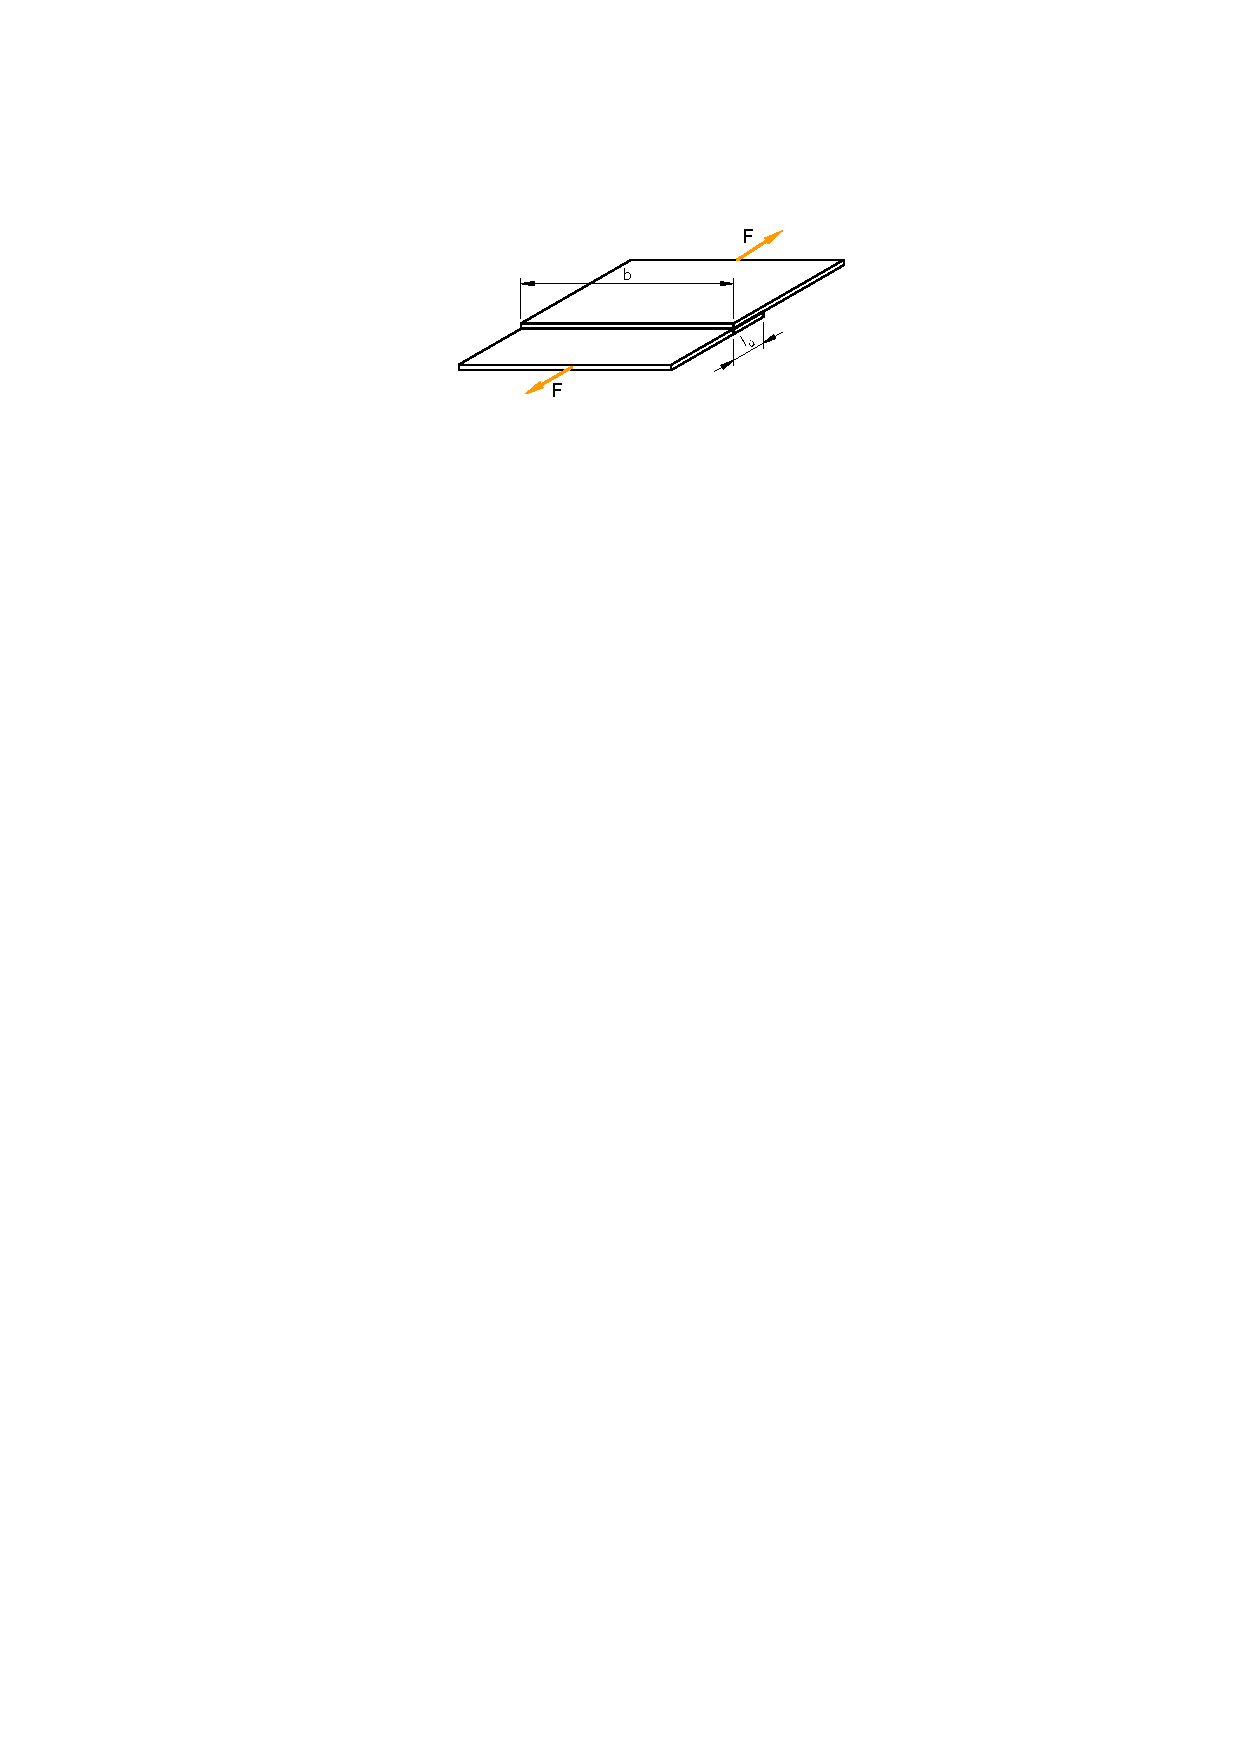
\includegraphics[width=.6\columnwidth]{graphics/klebe_scher}
		\end{center}
		
		Der Belastungsfall Scherung ist konstruktiv anzustreben! Überschlagsrechnung mit gemittelten Spannungen:
		\begin{equation*}
			\tau = \frac{F}{b \cdot l_{"u}} \leq \tau_{\text{zul}} = \frac{\tau_B}{S_B}
		\end{equation*}
		Diverse Abminderungsfaktoren kommen zum Tragen, sodass die Faustregel gilt:
		\begin{equation*}
			\tau_{B\text{,real}} \approx 0.1 \cdot \tau_B
		\end{equation*}
		Die optimale Überlappungslänge ist gegeben als:
		\begin{equation*}
			l_{"u\text{,opt}} = \frac{R_m \cdot t}{\tau_B}
		\end{equation*}
		und füt duktile metallische Werkstoffe:
		\begin{equation*}
			l_{"u\text{,opt}} = \frac{R_{0.2} \cdot t}{\tau_B}
		\end{equation*}
		mit $t$ als Fügeteildicke.
	% subsection: Scherbeanspruchung (end)
	\subsection{Schälbeanspruchung} % (fold)
		\begin{wrapfigure}{r}{.45\columnwidth}
			\vspace{-1.4cm}
			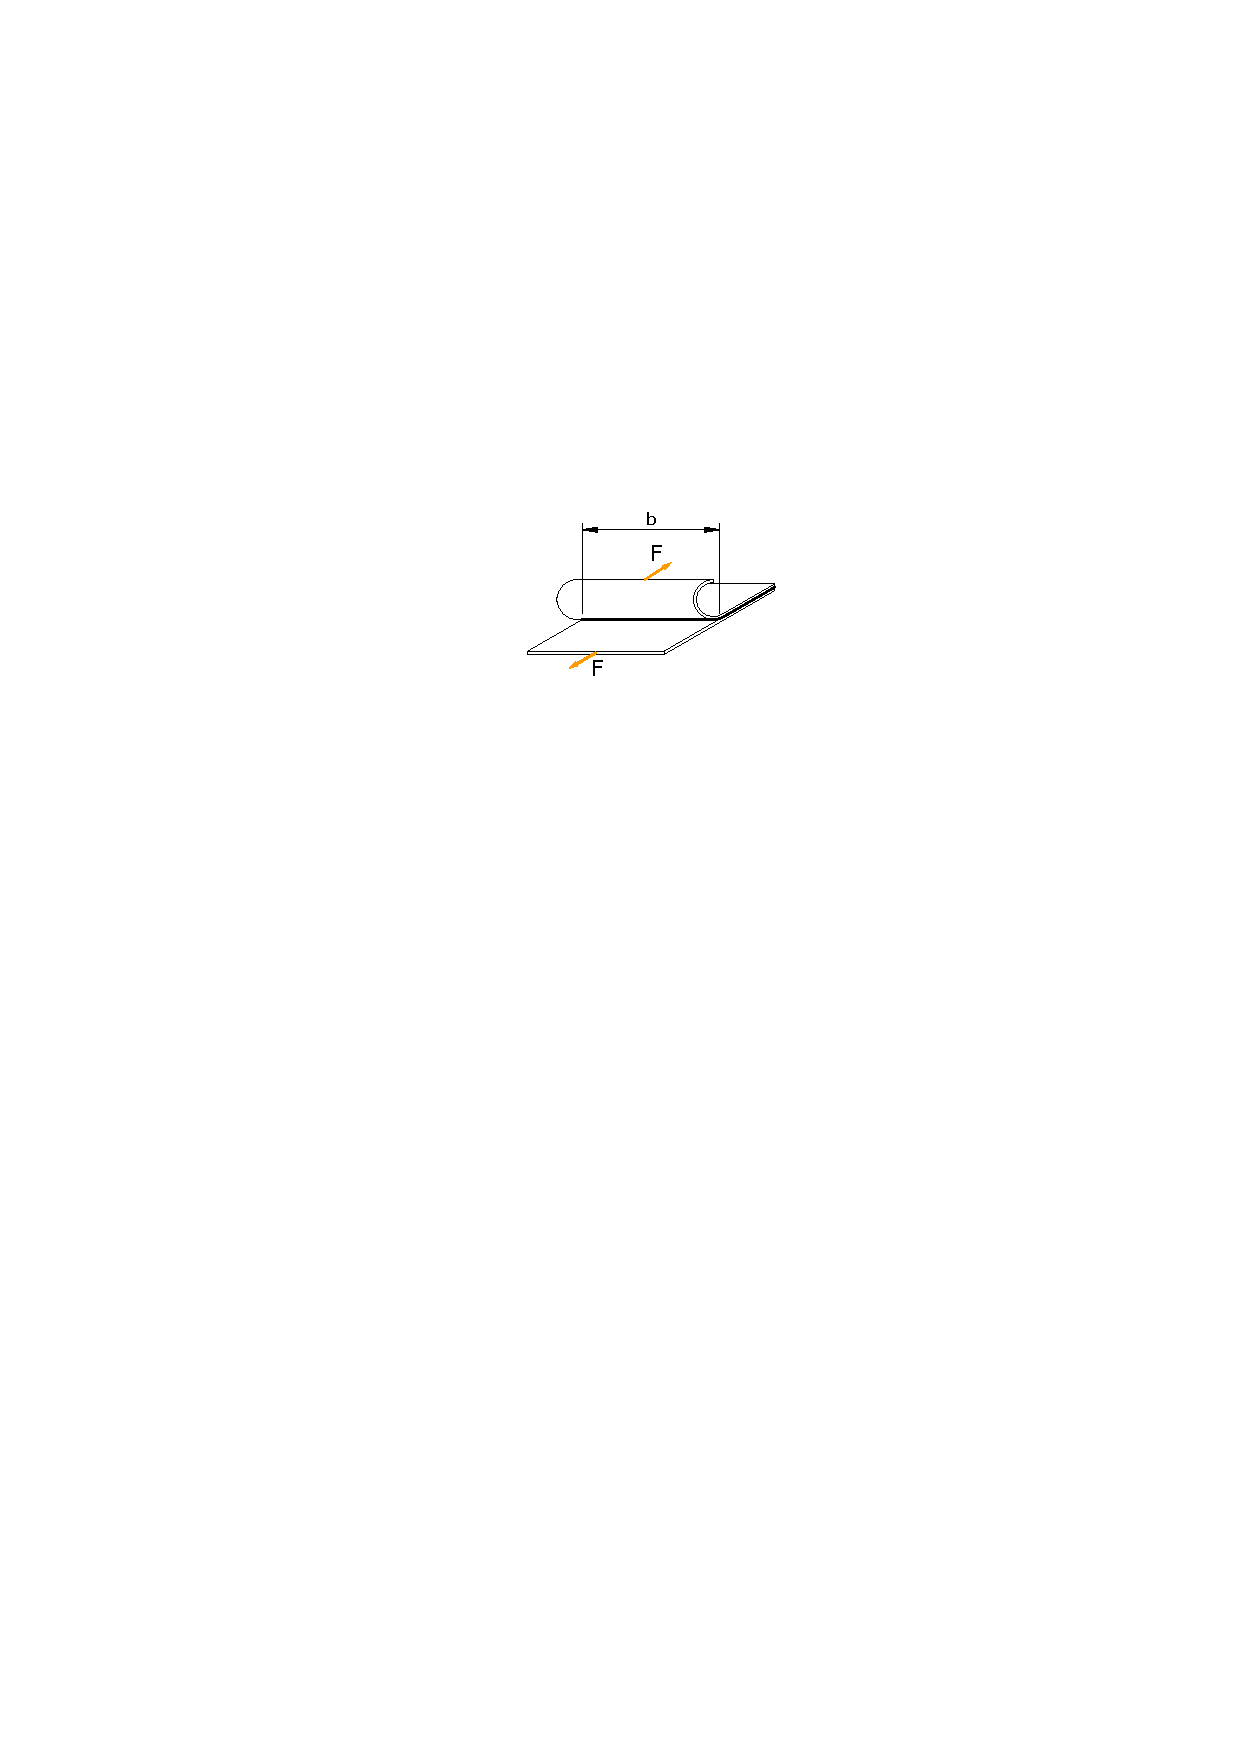
\includegraphics[width=.45\columnwidth]{graphics/klebe_schael}
		\end{wrapfigure}
		
		Dieser Belastungsfall ist der Un\-güns\-tigs\-te und deswegen konstruktiv mög\-lichst auszuschliessen.
		\begin{equation*}
			\sigma_x = \frac{F}{b \cdot \text{EH}} \leq \sigma_{\text{zul}} = \frac{\sigma_{\text{abs}}}{S_K}, \quad \text{EH: Einheitslänge \unit{\mm}}
		\end{equation*}
	% subsection: Schälbeanspruchung (end)
% section: Dimensionierung (end)
\section{Geometrie} % (fold)
	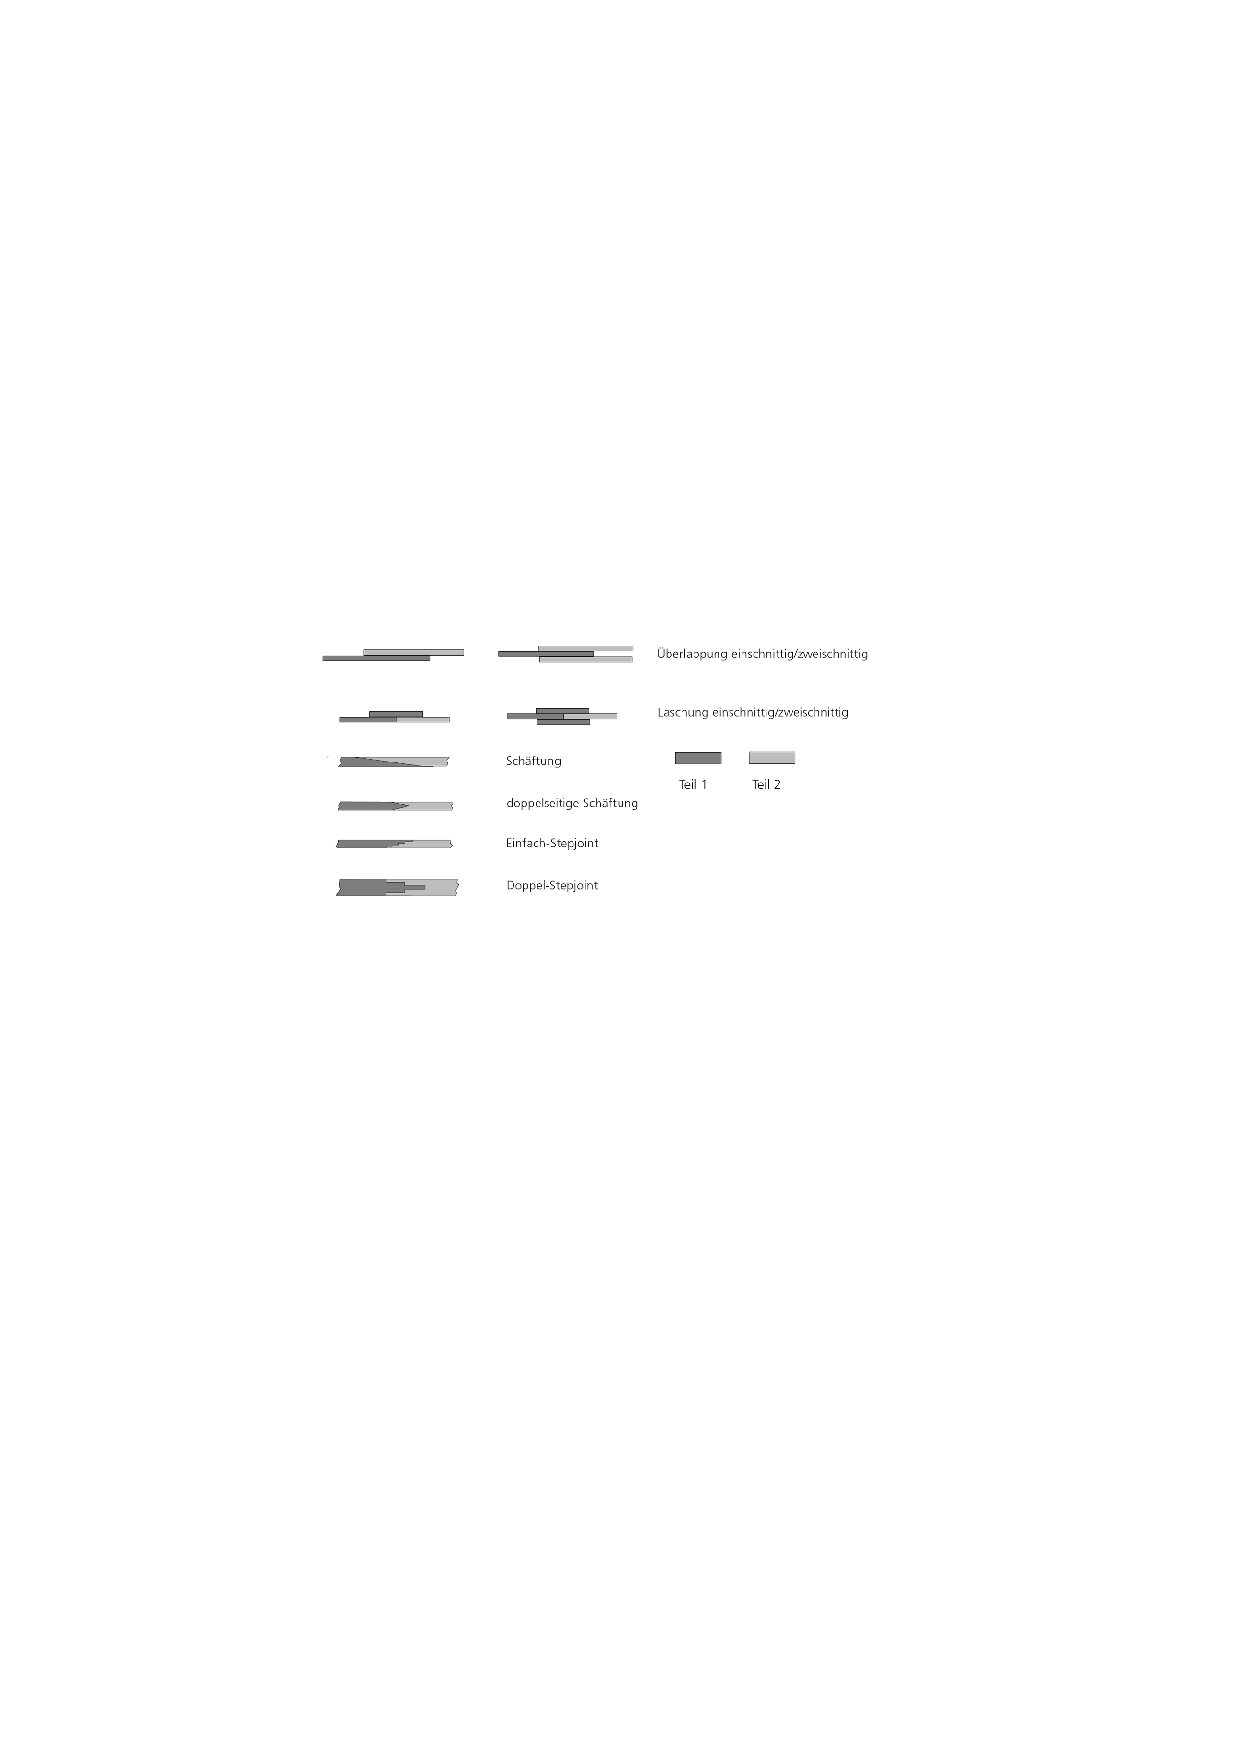
\includegraphics[width=\columnwidth]{graphics/klebverbindungen}
	
	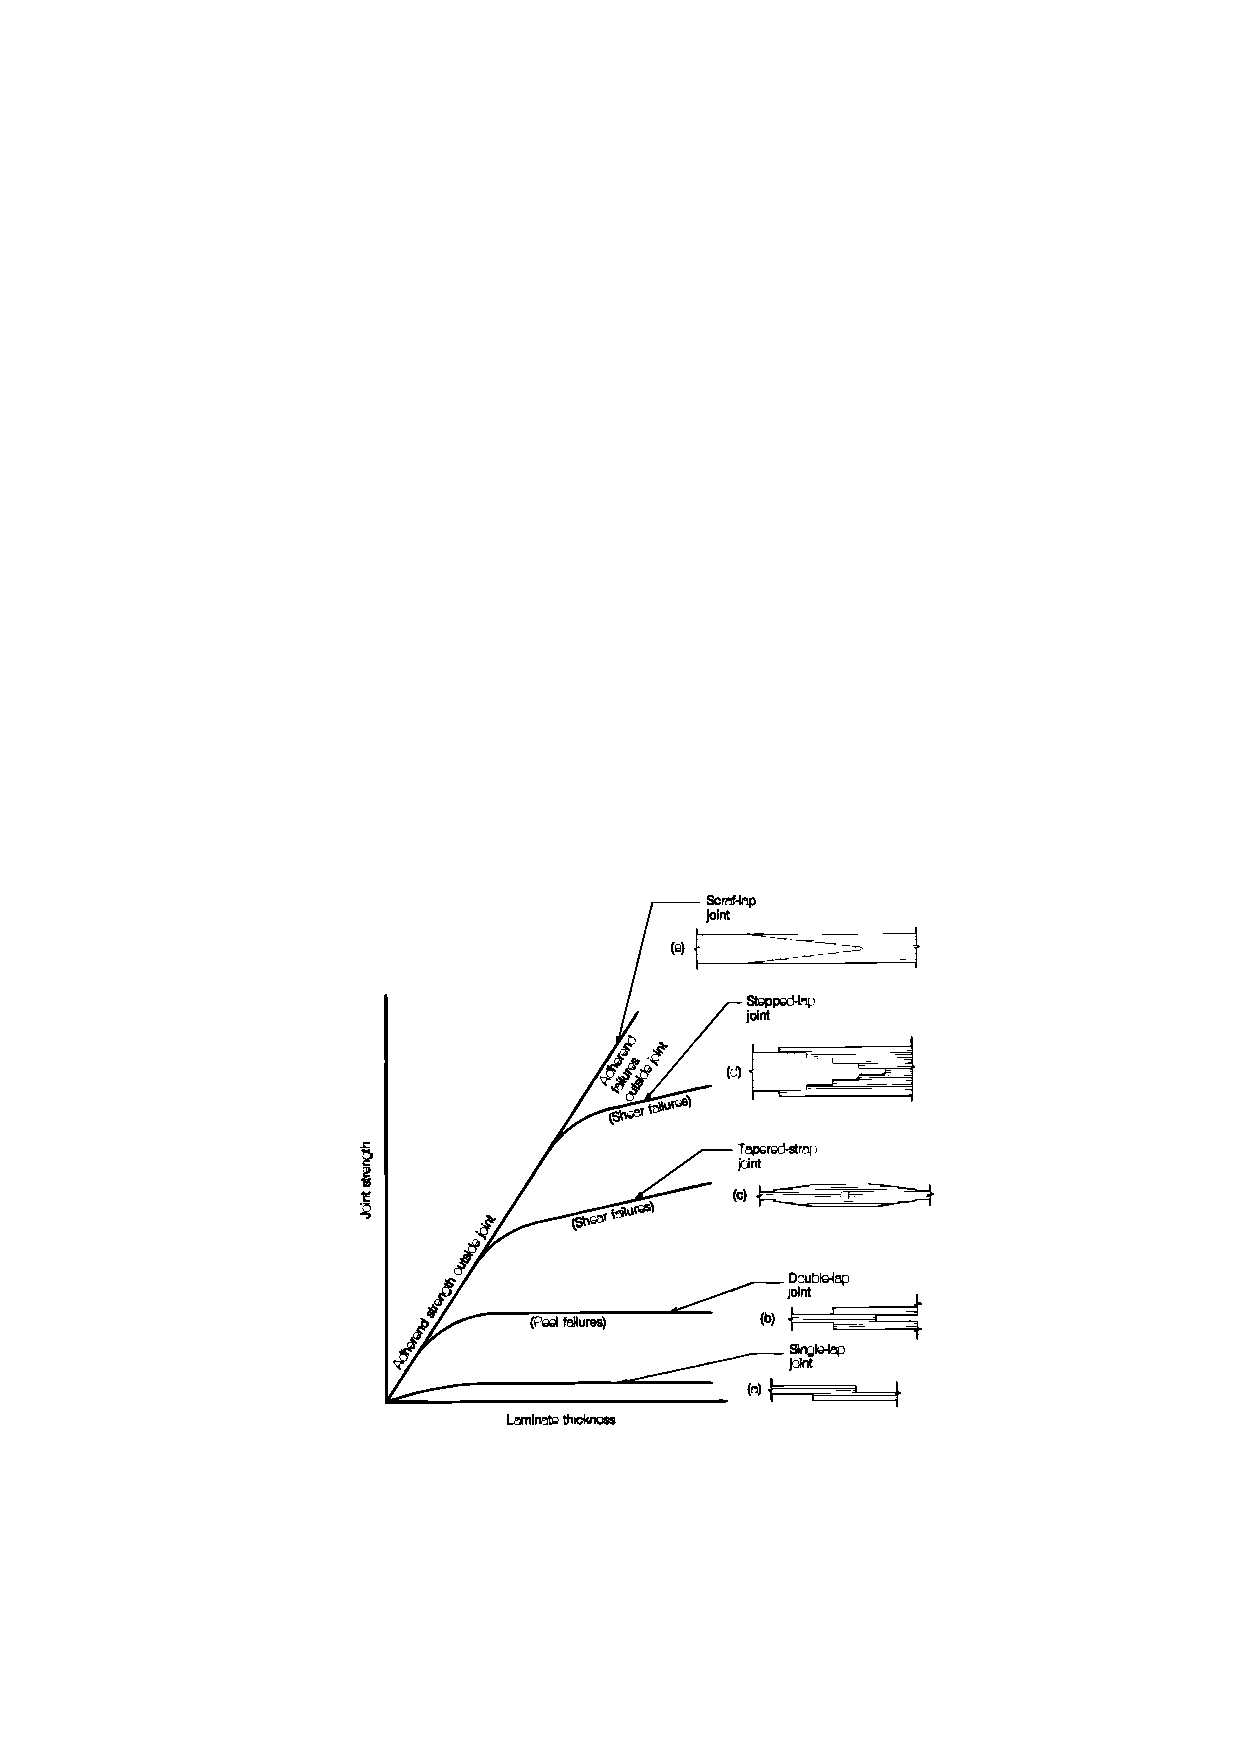
\includegraphics[width=\columnwidth]{graphics/klebefestigkeit}
% section: Geometrie (end)
\section{Klebefuge} % (fold)
	Schubwinkel in der Klebefuge ist gegeben durch:
	\begin{equation*}
		\tan(\gamma) = \frac{F_\text{schub}}{d_\text{Fuge}}
	\end{equation*}
% section: Klebefuge (end)